
\begin{center}
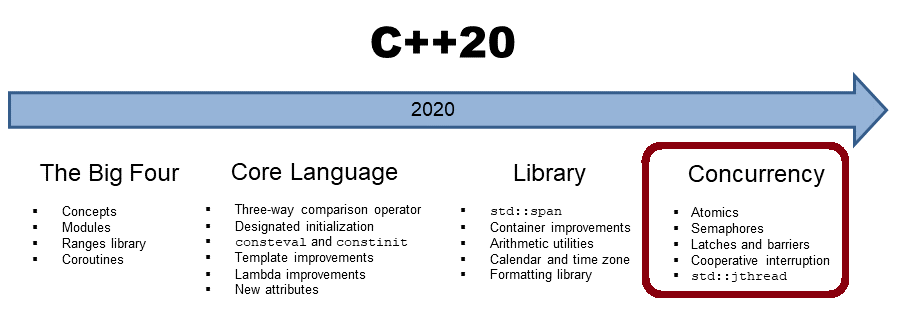
\includegraphics[width=1.0\textwidth]{content/2/chapter3/images/7.png}\\
\end{center}

\subsubsubsection{3.4.1\hspace{0.2cm} Atomics}

The class template std::atomic\_ref applies atomic operations to the referenced non-atomic object.
Concurrent writing and reading of the referenced object can take place, therefore, with no data race.
The lifetime of the referenced object must exceed the lifetime of the std::atomic\_ref. Accessing a subobject of the referenced object with std::atomic\_ref is not thread-safe.

According to \href{https://en.cppreference.com/w/cpp/atomic/atomic}{std::atomic}, std::atomic\_ref can be specialized and supports specializations for the built-in data types.

\begin{lstlisting}[style=styleCXX]
struct Counter {
	int a;
	int b;
};

Counter counter;

std::atomic_ref<Counter> cnt(counter);
\end{lstlisting}

With C++20, we get two atomic smart pointers that are partial specializations of std::atomic: there are std::atomic<std::shared\_ptr<T>> and std::atomic<std::weak\_ptr<T>>. Both atomic smart pointers guarantee that not only the control block, as in the case of \href{https://en.cppreference.com/w/cpp/memory/shared_ptr}{std::shared\_ptr}, is thread-safe, but also the associated object.

std::atomic gets more extensions. C++20 provides specializations for atomic floating-point types.
This is quite convenient when you have a concurrently incremented floating-point type.

A value of type \href{https://en.cppreference.com/w/cpp/atomic/atomic_flag}{std::atomic\_flag} is a kind of atomic boolean. It has a cleared and set state. For simplicity reasons, I call the clear state false and the set state true. The clear() member function enables you to set its value to false. With the test\_and\_set() member function, you can set the value to true and get the previous value. There is no member function to ask for the current value. This will change with C++20, because std::atomic\_flag has a test() method.

Furthermore, std::atomic\_flag can be used for thread synchronization via the member functions notify\_one(), notify\_all(), and wait(). With C++20, notifying and waiting is available on all partial and full specializations of std::atomic and std::atomic\_ref. Specializations are available for bools, integrals, floats, and pointers.

\subsubsubsection{3.4.2\hspace{0.2cm} Semaphores}

Semaphores are a synchronization mechanism used to control concurrent access to a shared resource. A counting semaphore, such as the one which was added in C++20, is a special semaphore whose inital counter is bigger than zero. The counter is initialized in the constructor. Acquiring the semaphore decreases the counter, and releasing the semaphore increases the counter. If a thread tries to acquire the semaphore when the counter is zero, the thread blocks until another thread increments the counter by releasing the semaphore.


\subsubsubsection{3.4.3\hspace{0.2cm}  Latches and Barriers}

Latches and barriers are straightforward thread synchronization mechanisms that enable some threads to block until a counter becomes zero. What are the differences between these two mechanisms to synchronize threads? You can use a std::latch only once, but you can use a std::barrier more than once. A std::latch is useful for managing one task by multiple threads; a std::barrier is useful for managing repeated tasks by multiple threads. Furthermore, a std::barrier can adjust the counter in each iteration.

The following is based on a code snippet from proposal \href{http://www.open-std.org/jtc1/sc22/wg21/docs/papers/2014/n4204.html}{N4204}. I fixed a few typos and reformatted it.

\noindent
Thread-synchronization with a std::latch
\begin{lstlisting}[style=styleCXX]
void DoWork(threadpool* pool) {

	std::latch completion_latch(NTASKS);
	for (int i = 0; i < NTASKS; ++i) {
		pool->add_task([&] {
			// perform work
			...
			completion_latch.count_down();
		});
	}
	// Block until work is done
	completion_latch.wait();
}
\end{lstlisting}

The counter of the std::latch completion\_latch is set to NTASKS (line 3). The thread pool executes NTASKS jobs (lines 4 - 10). At the end of each job, the counter is decremented (line 8). The thread running function DoWork blocks in line 12 until all tasks have been finished.

\subsubsubsection{3.4.4\hspace{0.2cm} Cooperative Interruption}

Thanks to std::stop\_token, a std::jthread can be interrupted cooperatively.

\noindent
Interrupting a std::jthread
\begin{lstlisting}[style=styleCXX]
int main() {
	
	std::cout << '\n';
	
	std::jthread nonInterruptible([]{
		int counter{0};
		while (counter < 10){
			std::this_thread::sleep_for(0.2s);
			std::cerr << "nonInterruptible: " << counter << '\n';
			++counter;
		}
	});
	
	std::jthread interruptible([](std::stop_token stoken){
	int counter{0};
	while (counter < 10){
		std::this_thread::sleep_for(0.2s);
			if (stoken.stop_requested()) return;
			std::cerr << "interruptible: " << counter << '\n';
			++counter;
		}
	});
	
	std::this_thread::sleep_for(1s);
	
	std::cerr << '\n';
	std::cerr << "Main thread interrupts both jthreads" << std:: endl;
	nonInterruptible.request_stop();
	interruptible.request_stop();
	
	std::cout << '\n';
	
}
\end{lstlisting}

The main program starts two threads, nonInterruptible and interruptible (lines 5 and 14). Only thread interruptible gets a std::stop\_token, which it uses in line 18 to check if it is interrupted. The lambda immediately returns in case of an interruption. The call to interruptible.request\_stop() triggers the cancellation of the thread. Calling nonInterruptible.request\_stop() has no effect.

\begin{center}
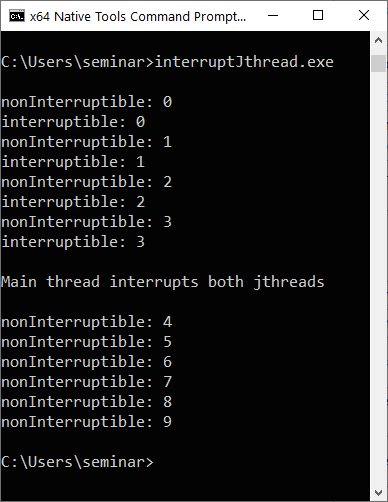
\includegraphics[width=0.6\textwidth]{content/2/chapter3/images/8.png}\\
Cooperative interruption of a thread
\end{center}

\subsubsubsection{3.4.5\hspace{0.2cm} std::jthread}

std::jthread stands for joining thread. std::jthread extends \href{https://en.cppreference.com/w/cpp/thread/thread}{std::thread} by automatically joining the started thread. std::jthread can also be interrupted.

std::jthread is added to the C++20 standard because of the non-intuitive behavior of std::thread. If a std::thread is still joinable, \href{https://en.cppreference.com/w/cpp/error/terminate}{std::terminate} is called in its destructor. A thread thr is joinable if neither thr.join() nor thr.detach() was called.

\noindent
Thread thr is still joinable
\begin{lstlisting}[style=styleCXX]
int main() {
	
	std::cout << '\n';
	
	std::cout << std::boolalpha;
	std::thread thr{[]{ std::cout << "Joinable std::thread" << '\n'; }};
	std::cout << "thr.joinable(): " << thr.joinable() << '\n';
	
	std::cout << '\n';
}
\end{lstlisting}

\begin{center}
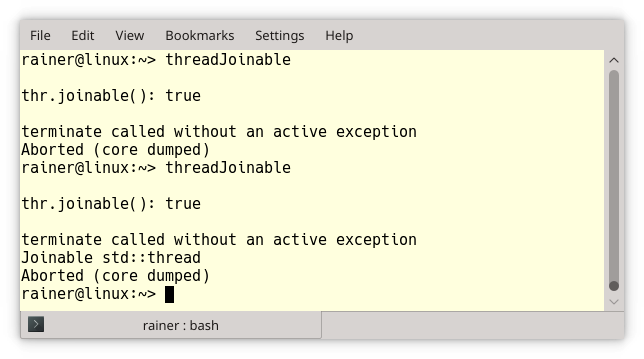
\includegraphics[width=0.8\textwidth]{content/2/chapter3/images/9.png}\\
std::terminate with a still joinable thread
\end{center}

Both executions of the program terminate. In the second run, the thread thr has enough time to display its message: “Joinable std::thread”.

In the modified example, I use std::jthread from the C++20 standard.

\noindent
Thread thr joins automatically
\begin{lstlisting}[style=styleCXX]
int main() {
	std::cout << '\n';
	
	std::cout << std::boolalpha;
	std::jthread thr{[]{ std::cout << "Joinable std::jthread" << '\n'; }};
	std::cout << "thr.joinable(): " << thr.joinable() << '\n';
	
	std::cout << '\n';
}
\end{lstlisting}

Now, thread thr automatically joins in its destructor if necessary.

\begin{center}
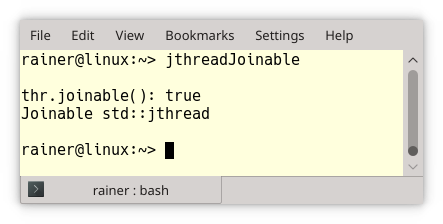
\includegraphics[width=0.8\textwidth]{content/2/chapter3/images/10.png}\\
Thread thr joins automatically
\end{center}

\subsubsubsection{3.4.6\hspace{0.2cm} Synchronized Outputstreams}

With C++20, we get synchronized outputstreams. What happens when more threads write concurrently to std::cout without synchronization?

\noindent
Unsynchronized writing to std::cout
\begin{lstlisting}[style=styleCXX]
void sayHello(std::string name) {
	std::cout << "Hello from " << name << '\n';
}

int main() {
	std::cout << "\n";
	
	std::jthread t1(sayHello, "t1");
	std::jthread t2(sayHello, "t2");
	std::jthread t3(sayHello, "t3");
	std::jthread t4(sayHello, "t4");
	std::jthread t5(sayHello, "t5");
	std::jthread t6(sayHello, "t6");
	std::jthread t7(sayHello, "t7");
	std::jthread t8(sayHello, "t8");
	std::jthread t9(sayHello, "t9");
	std::jthread t10(sayHello, "t10");
	
	std::cout << '\n';
}
\end{lstlisting}

You may get a mess.

\begin{center}
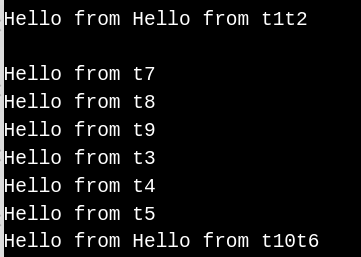
\includegraphics[width=0.8\textwidth]{content/2/chapter3/images/11.png}\\
Unsynchronized writing to std::cout
\end{center}

Switching from std::cout in the function sayHello to std::osyncstream(std::cout) turns the mess into a harmony.

\noindent
Synchronized writing to std::cout
\begin{lstlisting}[style=styleCXX]
void sayHello(std::string name) {
	std::osyncstream(std::cout) << "Hello from " << name << '\n';
}
\end{lstlisting}

\begin{center}
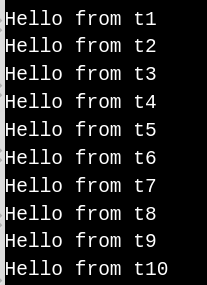
\includegraphics[width=0.4\textwidth]{content/2/chapter3/images/12.png}\\
Synchronized writing to std::cout
\end{center}
